\documentclass[11pt,a4paper]{article}
\usepackage{fullpage}
\usepackage[utf8]{inputenc}
\usepackage[french]{babel}
\usepackage[T1]{fontenc}
\usepackage{amsmath}
\usepackage{amsfonts}
\usepackage{amssymb}
\usepackage{amsthm}
\usepackage{stmaryrd}
\usepackage[all]{xy}
\usepackage{fancybox}
\usepackage{tikz}
\usepackage{pgfplots}
\usepackage{framed}
\usepackage{lmodern}
\usepackage{xcolor}
\usepackage{comment}
\usepackage{arydshln}
%\usepackage[shell]{gnuplottex}
\usepackage{fancyvrb}
\usepackage{xcolor}
\usepackage{cite}
\usepackage[outline]{contour}
\usepackage{eso-pic}
\usepackage{titlepic}
\usepackage{fancyhdr}
\usepackage{listings}

\newcommand{\HRule}{\rule{\linewidth}{0.1mm}}
\newcommand{\blap}[1]{\vbox to 0pt{#1\vss}}
\newcommand\AtUpperLeftCorner[3]{%
  \put(\LenToUnit{#1},\LenToUnit{\dimexpr\paperheight-#2}){\blap{#3}}%
}
\newcommand\AtUpperRightCorner[3]{%
  \put(\LenToUnit{\dimexpr\paperwidth-#1},\LenToUnit{\dimexpr\paperheight-#2}){\blap{\llap{#3}}}%
}

\lstset { %
    language=C++,
    basicstyle=\footnotesize,% basic font setting
    commentstyle=\color{green}, % comment color
    keywordstyle=\color{blue}, % keyword color
    stringstyle=\color{gray} % string color
}

\title{TV-L1 Optical Flow Estimation}
\author{Kevin Trancho}
\date{Master Image - Année 2018-2019}

\begin{document}

\begin{titlepage}
\begin{sffamily}
\begin{center}

\begin{minipage}{0.49\textwidth}
\begin{flushleft}

\includegraphics[width=0.8\columnwidth]{UPEM_LOGO.png}
\end{flushleft}
\end{minipage}
\begin{minipage}{0.49\textwidth}
\begin{flushright}

\includegraphics[width=0.45\columnwidth]{MONGE_LOGO.png}
\end{flushright}
\end{minipage}

~\\[1.25cm]


\HRule \\[0.22cm]
    { \begin{Huge} Système solaire\\[0.42cm]\end{Huge}\begin{Large}Projet de synthèse d'images\\[0.22cm]\end{Large}}
 \HRule \\[0.62cm]

\vspace*{1\baselineskip}

{\begin{Large}Kevin \textsc{Trancho} et Victor \textsc{Veillerette}\\[0.20cm]\end{Large}}
{\begin{large}Master Informatique 2\up{ème} année\\[0.10cm]\end{large}}
{\begin{large}Spécialité Sciences de l'image\\[0.10cm]\end{large}}
{\begin{large}Année 2018 - 2019\\[1.5cm]\end{large}}

%~\\[1cm]

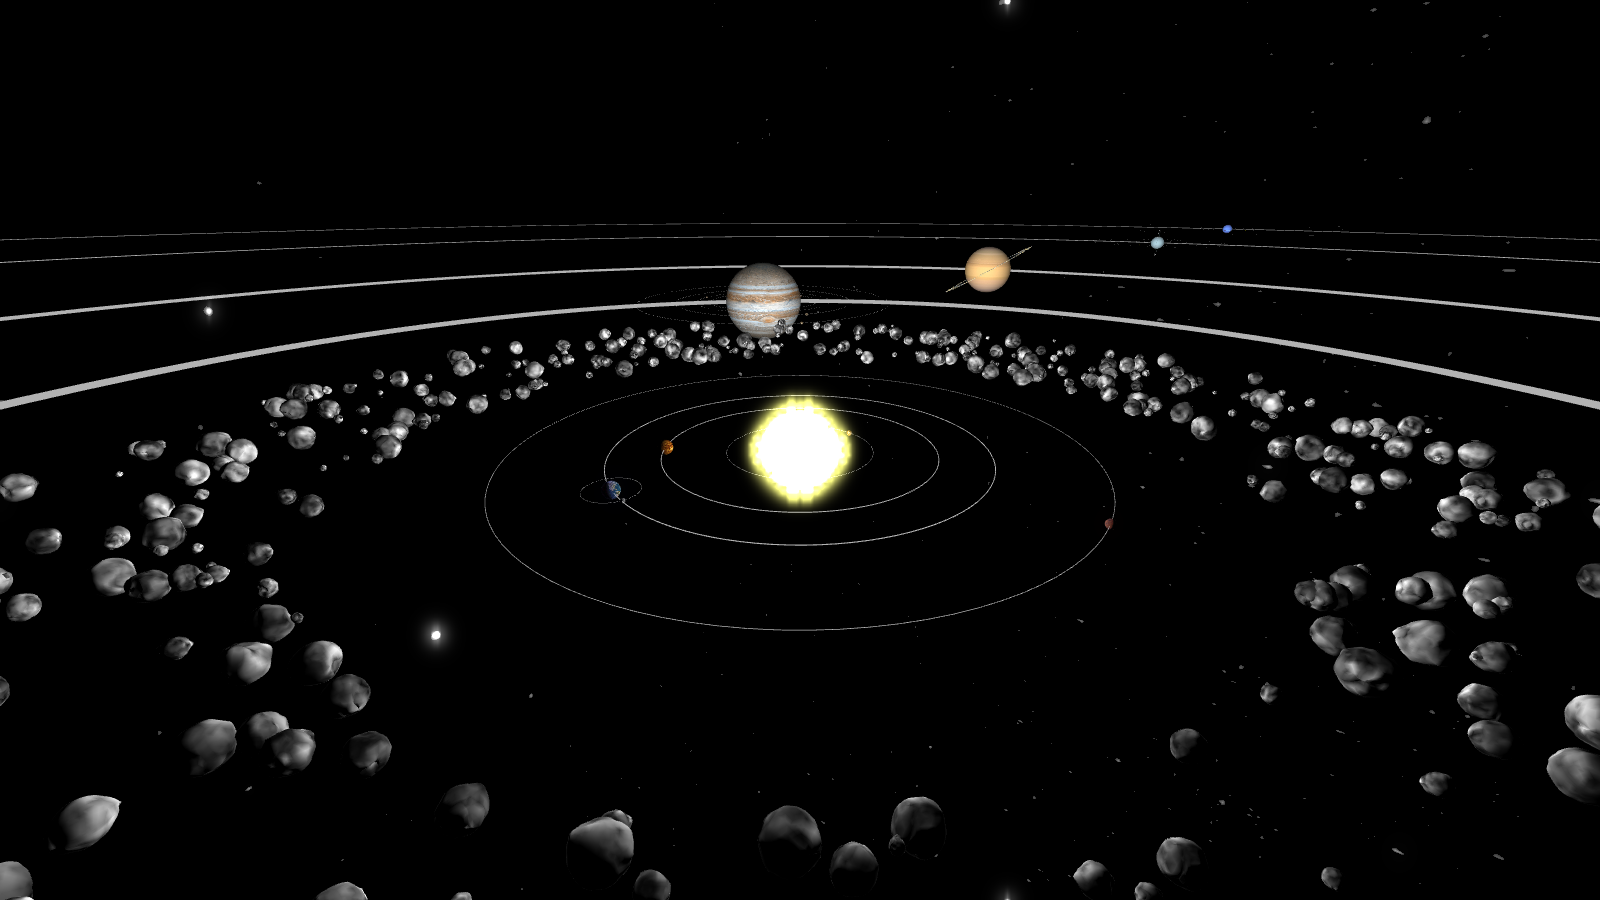
\includegraphics[width=0.95\columnwidth]{First.png}

~\\[1cm]

\end{center}
\end{sffamily}
\end{titlepage}

\newpage
\tableofcontents
\newpage

\section{Architecture}

L'architecture que nous proposons est la suivante :
\begin{figure}[h!]
\centering
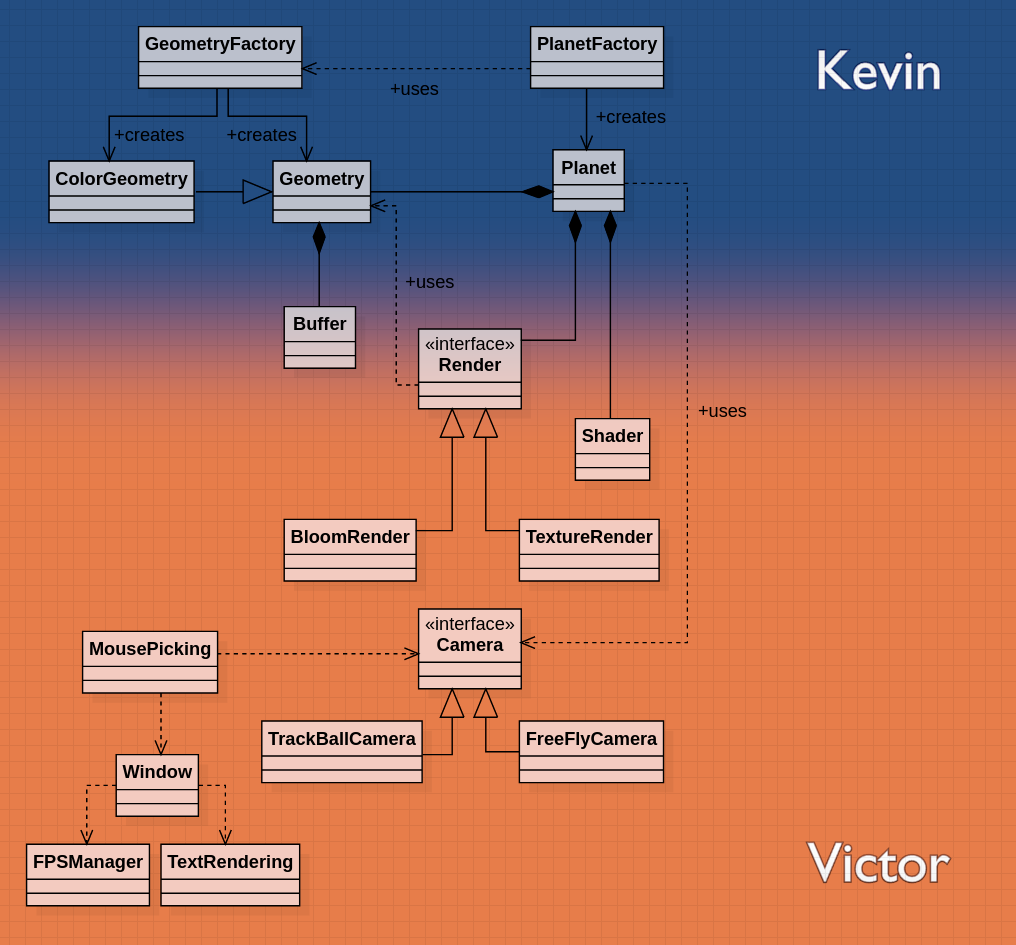
\includegraphics[width=0.99\columnwidth]{Archi_gestion_de_projet.png}
\end{figure}

Dans la séparation des tâches, Kevin était principalement chargé de gérer que qui touche à la géométrie et gestion des planètes et Victor avait pour rôle principal de s'occuper de la partie qui s'intéresse au rendu, vue depuis une caméra et gestion des shaders.

\section{Fonctionnalités basiques}
\subsection{Surcouches à OpenGL et SDL}
Plusieurs classes permettent de gérer plus facilement les fonctions OpenGL/SDL de base niveaux :\\
\begin{itemize}
\item La classe \textbf{Buffer} permet de gérer les différents \textsc{vbo}, \textsc{vao}, \textsc{ibo}.
On lui fournit un ensemble de sommets (\textsc{vertex}, \textsc{normal}, \textsc{textureCoord}) et de faces et il se charge automatiquement de générer les buffers en mémoire GPU
et à les remplir correctement. Cela permet de simplifier grandement la création des géométries.\\
\item La classe \textbf{TextureRender} permet de charger une image à partir d'un path et de correctement remplir les
textures du GPU et d'envoyer automatiquement les textures au bon endroit dans les shaders.\\
\item La classe \textbf{Shader} permet l'utilisation simplifiée des shaders en retrouvant automatiquement l'emplacement 
des variables uniformes grâce à une map :
\begin{lstlisting}
void uniformMatrix(std::string key, glm::mat4 & mat);
void uniformValue(std::string key, GLfloat value);
void uniformVector(std::string key, glm::vec4 vec);
\end{lstlisting}

\item Enfin, les classes \textbf{Window} et \textbf{FPSManager} englobent les fonctions SDL et permettent :
	\begin{itemize}
	\item D'ouvrir/fermer une fenêtre
	\item De gérer le clavier
	\item De lancer la boucle principale de l'application en utilisant deux lambdas : une pour la gestion des événements
	et l'autre pour le rendu. Cette boucle s'assure en interne que le nombre de FPS soit constant (option réglable) :
	\begin{lstlisting}
void run(std::function<bool(SDL_Event *)> play, std::function<void()> draw);
	\end{lstlisting}
	\end{itemize}
\end{itemize}

\subsection{Caméras}
L'interface \textbf{Camera} permets de généraliser le principe et de rendre facile le changement de caméra pendant l'execution. Elle demande l'implémentation suivante :
\begin{lstlisting}
virtual glm::mat4 getViewMatrix() const = 0;
virtual glm::vec4 getPosition() const = 0;
virtual void gestEvent(SDL_Event *event) = 0;
\end{lstlisting}
Deux caméras ont été implémentées : la \textbf{TrackBall Camera} qui permet de tourner autours d'un object (planètes, satellites, astéroides) ainsi que la \textbf{Freefly Camera} qui permet de se déplacer dans toutes les directions à la manière d'une caméra FPS.

\subsection{Géométrie}

Nous proposons un module \textbf{Geometry} permettant de garder en mémoire une forme générée : sommets et faces.
La création des différentes primitives classiques est proposée à l'aide de \textbf{GeometryFactory}. Celle-ci permet principalement de générer les UV-sphères pour les planètes, les tores pour les trajectoires, la forme d'une Skybox pour le ciel étoilé, mais aussi les astéroïdes.

\subsection{Planètes}
\subsubsection{Planet}

La classe \textbf{Planet} fait le lien entre la géométrie et le rendu. C'est-à-dire qu'elle connaît une unique géométrie à laquelle on peut ajouter des textures ou d'autres composants de rendu tels que des anneaux, une atmosphère par exemple.
L'autre idée du module Planet est d'être générique et permettre la récursivité. C'est-à-dire qu'une planète peut aussi bien être un soleil, un satellite ou un astéroïde.

\subsubsection{PlanetFactory}

La classe \textbf{PlanetFactory} a pour fonction principale de lire la recette de fabrication d'une planète, soleil, ceinture d'astéroïdes depuis un fichier : le système solaire proposé est chargé depuis \verb!assets/solar_system!.

\subsection{Astéroïdes}
\subsubsection{Ico-sphère et génération}

Nous avons choisi de générer les astéroïdes, l'idée était de le faire depuis une sphère. Mais les UV-sphères ne permettant pas une déformation homogène de la surface (à cause des pôles). Nous proposons l'\textbf{Ico-sphère}. À noter que l'Ico-sphère est aussi utilisée pour l'atmosphère des planètes et donne de meilleurs résultats qu'une UV-sphère.

Pour construire une Ico-sphère nous construisons un géodésique simple (ici les sommets sont construits à partir de 3 rectangles orthogonaux). L'étape suivante est de le subdiviser puis projeter chaque sommet sur une sphère (renormalisation à distance 1 de l'origine).
Pour fabriquer un astéroïde, l'idée est de générer aléatoirement des potentiels (ici sources avec une force positive ou négative), puis de calculer la somme des déformations de chaque sommet vers un potentiel donné selon un coefficient de déformation fixé.
L'augmenter le nombre de potentiels va augmenter le nombre de cabossages de la forme obtenue et augmenter le coefficient de déformation va augmenter les étirements de la forme mais aussi les irrégularités.

Sur la figure suivante nous illustrons premièrement le géodésique, puis une subdivision de celui-ci.
Ensuite sont affiché une ico-sphère et deux astéroïdes (un cabossé par 200 potentiels pour une déformation de 10 et l'autre 500 potentiels et déformation 20).

\begin{figure}[h!]
\centering
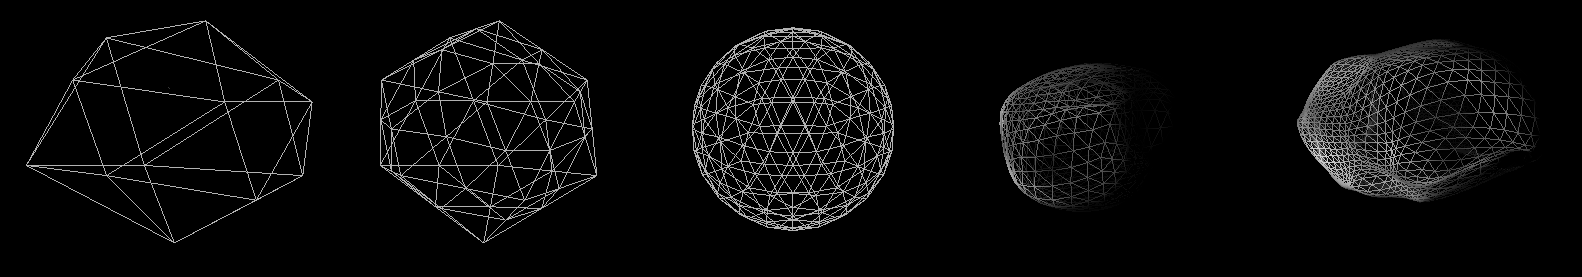
\includegraphics[width=0.99\columnwidth]{img/ico.png}
\end{figure}

\subsubsection{Ceinture d'astéroïdes}

La ceinture d'astéroïdes est obtenue par génération aléatoire de tailles, rotation, positions aléatoire pour des valeurs dans des intervalles donnés pour un ensemble d'astéroïdes générés dans une zone définie par un anneau. Ici si on demande $N$ astéroïdes, on générera de l'ordre de $3 \log_2\left(N\right)$ géométries différentes d'astéroïdes.

\section{Fonctionnalités supplémentaires}

\subsection{Mouse picking}
On souhaite qu'au clic de la souris sur une planète, notre caméra se déplace vers celui-ci. Pour cela, on va lancer
un rayon de la caméra passant par le point du clic et on cherche alors à voir si il intersecte un des objets de notre scène.\\
C'est le rôle de la classe \textbf{MousePicking}. Elle utilise l'algorithme suivant :
\begin{enumerate}
\item Transformations en coordonnées homogènes clippées ([-1;1], [-1;1], -1, 1) :
\begin{lstlisting}
vec4 coords = ((2 * x) / W - 1, (1 - 2 * y / H))
\end{lstlisting}

\item Transformations en coordonées de l'espace view :
\begin{lstlisting}
vec4 coordsView = vec4(vec2(inverse(projectionMatrix) * coords), -1, 0)
\end{lstlisting}

\item Transformations en coordonnées de l'espace monde :
\begin{lstlisting}
vec3 final = inverse(ViewMatrix) * coordsView
\end{lstlisting}
\end{enumerate}
Il est maintenant possible de vérifier l'intersection de notre rayon (qui part de la caméra) avec les objets de notre scène pour déterminer si on clique sur un élément. Ici on considèrera uniquement le plus proche objet qui intersecte.

\subsection{Rendu de texte}

On a souhaité faire un mécanisme de rendu de texte simple pour permettre d'afficher les FPS à l'écran par exemple. \\
Nous avons choisi la technique des \textbf{bitmap font}. On a donc généré la texture suivante à partir de la police Arial :
\begin{figure}[h!]
\centering
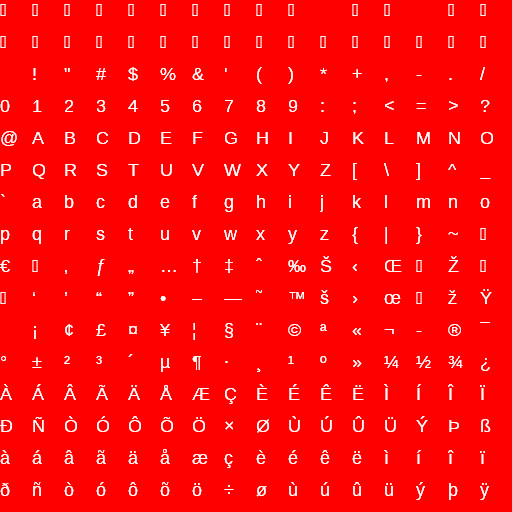
\includegraphics[width=0.25\columnwidth]{img/Arial.jpg}
\end{figure}

Lors du rendu, on dessine un rectangle à l'écran pour chaque lettre à écrire et on utilise les bonnes coordonnées de notre texture en fonction de la lettre à dessiner :
\begin{lstlisting}
float ux = (car % 16) / 16
float uy = (car / 16) / 16
\end{lstlisting}
On rends ensuite la couleur rouge transparente dans notre shader pour finaliser le dessin. On obtient par exemple :
\begin{figure}[h!]
\centering
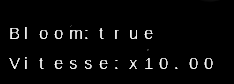
\includegraphics[width=0.25\columnwidth]{img/text.png}
\end{figure}

\subsection{Anti-Aliasing MSAA}
Nous nous sommes vite confrontés aux problèmes de crénelage mais surtout de la visualisation lointaine des petits objets (trajectoires).\\

Pour cela, nous avons opté pour le multisampling (MSAA) à 4 points. Pour cela, on crée un framebuffer que l'on associe à 
une texture \textsc{GL\_TEXTURE\_2D\_MULTISAMPLE}. On effectue le rendu grâce à un multisample renderbuffer associé.\\

Pour finir, on résoud le problème de la sélection en passant par un deuxième framebuffer qui sélectionne le point le plus proche : (\textsc{GL\_NEAREST}).
\begin{figure}[h!]
\centering
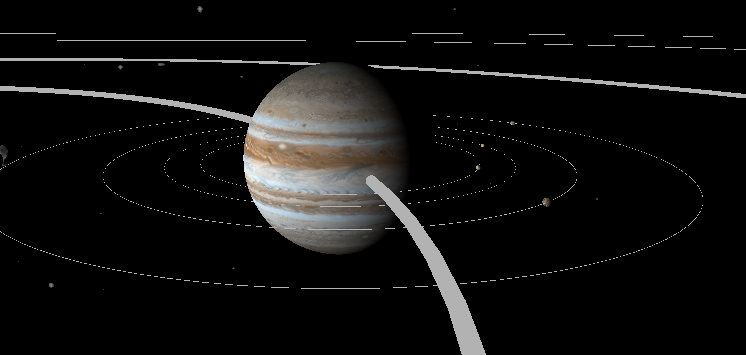
\includegraphics[width=0.70\columnwidth]{img/a.png}
\caption{Problème d'aliasing et de visualisation des objets fins}
\end{figure}

\begin{figure}[h!]
\centering
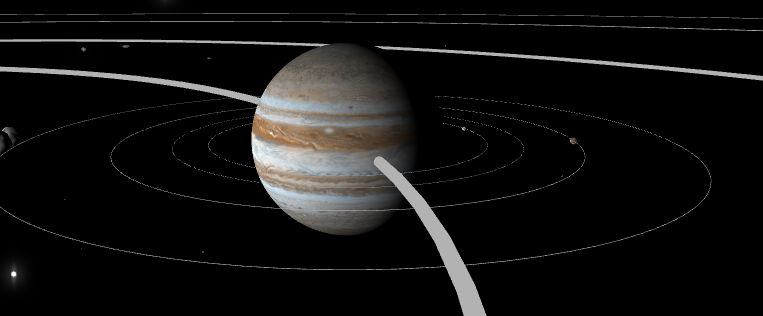
\includegraphics[width=0.70\columnwidth]{img/aa.png}
\caption{On a bien amélioré la qualité de rendu avec du MSAA 4x}
\end{figure}

On observe une baisse de performance d'environ 25\% pour une résolution 1920/1080, et une baisse de 35\% pour du MSAA 8x avec la même résolution.

\subsection{Bloom Effect}

On s'est également appercu que le rendu du soleil ne donnait vraiment pas l'impression d'une source lumineuse :\\
L'idée de l'algorithme est alors le suivant :\\
\begin{enumerate}
\item On effectue un rendu de notre scène standard avec deux sorties : la couleur normale et la couleur bright qui devra s'illuminer :
\begin{lstlisting}
layout (location = 0) out vec3 fFragColor;
layout (location = 1) out vec3 fBrightColor;
\end{lstlisting}
\item On effectue plusieurs itérations de flou gaussien (en deux étapes) sur la texture bright de notre scène.
\item On combine les deux pour obtenir le rendu final
\end{enumerate}
\begin{figure}[h!]
\centering
\begin{tabular}{l|c|c|c|}
    & bright color & 4 itérations & 16 itérations \\
   & 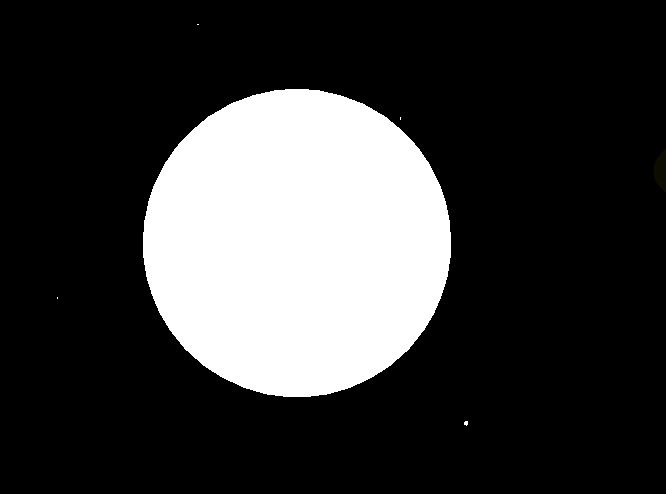
\includegraphics[width=0.30\columnwidth]{img/b1.png} & 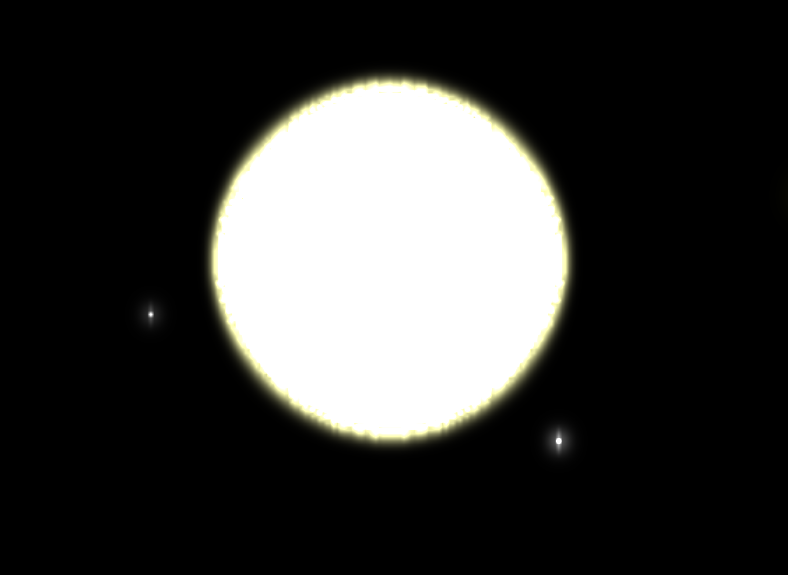
\includegraphics[width=0.30\columnwidth]{img/b4.png} & 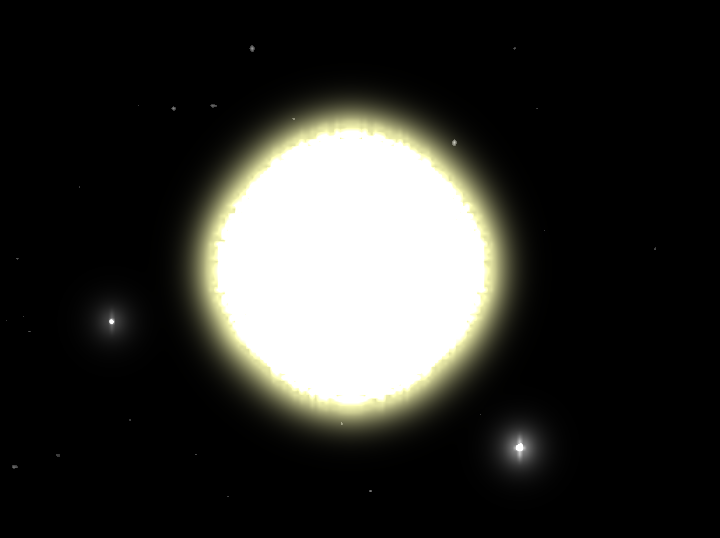
\includegraphics[width=0.30\columnwidth]{img/b16.png}  \\
\end{tabular}
\caption{Evolution de l'algorithme avec 4 et 16 itérations }
\end{figure}

\begin{figure}[h!]
\centering
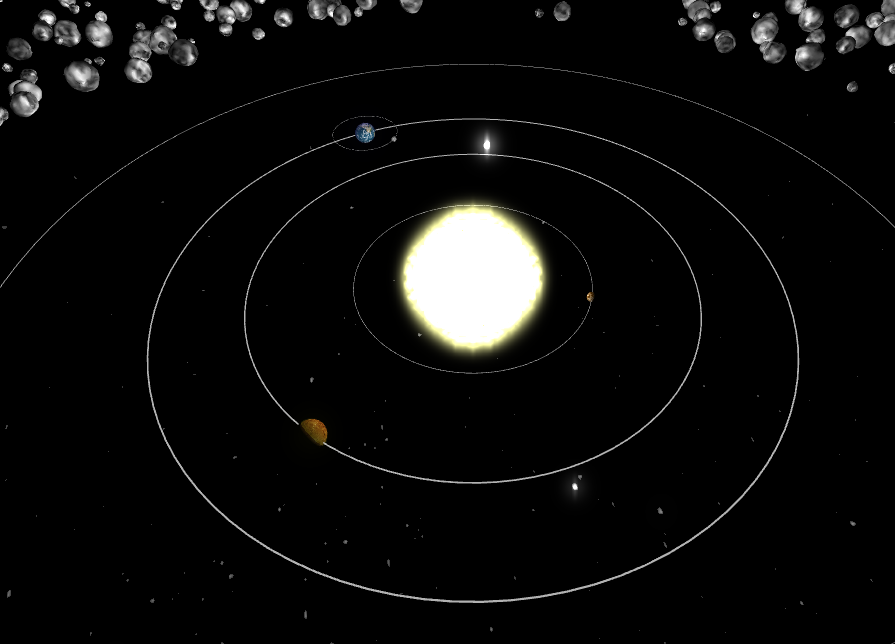
\includegraphics[width=0.60\columnwidth]{img/b.png}
\caption{Le rendu avec bloom et \textsc{msaa} est beaucoup plus satisfaisant.}
\end{figure}

\newpage
\section{Manuel}

\subsection{Compilation et exécution}

Pour compiler l'application :
\begin{lstlisting}
	mkdir build
	cd build
	cmake ..
	make
\end{lstlisting}
Pour lancer l'application :
\begin{lstlisting}
	./app/main
\end{lstlisting}
Si besoin, utiliser le mode de compatibilité mesa :
\begin{lstlisting}
	MESA_GL_VERSION_OVERRIDE=3.3 ./app/main
\end{lstlisting}

\subsection{Interface}

Le système solaire est alors chargé et affiché à l'écran. On peut se déplacer grâce à la souris et au clavier. Pour déplacer
l'angle de vue, il faut laisser enfoncé le clic gauche et bouger la souris.\\
Le tableau suivant résume les touches utiles :\\

\def\arraystretch{1.5}
\begin{figure}[h!]
\centering
\begin{tabular}{c|l}
    \hline
	\textbf{Touche} & \textbf{Description} \\ \hline
   	ESC		& Sortir de l'application \\ \hline
   	TAB		& Afficher les meshs \\ \hline
   	C		& Changer de caméra entre \textsc{trackball} et \textsc{freefly} \\ \hline
   	B		& Activer ou Désactiver le bloom et le MSAA \\ \hline
   	SPACE		& Arrêter/Relancer le temps\\ \hline
   	Flèche gauche	& Ralentir le temps \\ \hline
   	Flèche droite 	& Accélérer le temps \\ \hline
   	Souris + ZQSD	& Déplacer la caméra \\ \hline
   	Clic sur un objet & Déplacer la caméra vers cet objet \\ \hline
\end{tabular}
\caption{Manuel d'utilisation}
\end{figure}

\subsection{Fichiers de création de planètes}

\subsubsection{Création}

Pour démarrer une création, il y a deux possibilités : créer l'entité ou la charger depuis un fichier externe. Il est possible de créer un satellite récursivement avec la même syntaxe en donnant simplement l'attribut satellite.

Pour charger depuis un fichier externe :
\begin{verbatim}
load [PATH]
\end{verbatim}
ou générer la planète avec une syntaxe de la forme :
\begin{verbatim}
create [TYPE]
    [ATTRIBUT] [VALUES]
    [ATTRIBUT] [VALUES]
    ...
    [ATTRIBUT] [VALUES]
    satellite create [TYPE]
        [SATELLITE-ATTRIBUT] [VALUES]
        ...
    end
    ...
    satellite load [PATH]
    ...
end
\end{verbatim}
\newpage
Les différentes valeurs pour type sont les suivantes:
\begin{center}
\begin{tabular}{c|l}
    \hline
	\textbf{Type} & \textbf{Description} \\ \hline
   	\verb!Planet! & création d'une planète \\ \hline
   	\verb!Sun! & création d'un soleil \\ \hline
   	\verb!Asteroid-ring! & génération d'une ceinture d'astéroïdes \\ \hline
   	\verb!Obj! & suivi du chemin du .obj à charger \\ \hline
\end{tabular}
\end{center}

À noter que les attributs donnés pour \verb!Planet! sont aussi valables pour \verb!Sun! et \verb!Obj!.

\subsubsection{Attributs Planète}

\begin{verbatim}
create [Planet | Sun | Obj [PATH]]
    diameter [FLOAT: diamètre de la planète en km]
    parent-distance [FLOAT: distance au parent en km]
    orbital-period [FLOAT: période de rotation autours du parent en jours]
    rotation-period [FLOAT: période de rotation sur elle-même en heures]
    texture [PATH: chemin de la texture]
    texture-day [PATH: chemin de la texture principale]
    texture-night [PATH: chemin de la texture vue sur l'ombre]
    clouds [PATH: chemin de la texture en rotation en surface]
    ring [FLOAT: diamètre de l'anneau]
    color [FLOAT: couleur unie de la planète]
    ringtexture [PATH: chemin de la texture de l'anneau]
    ringalpha [PATH: chemin de la texture pour le canal alpha de la texture]
    ringangle [FLOAT: angle d'inclinaison de l'anneau]
    atmosphere [FLOAT: taille de l'atmosphère]
    atmosphereColor [vec3: couleur de l'atmosphère]
    satellite [GENERATION COMMAND: recette de fabrication du satellite]
end
\end{verbatim}

\subsubsection{Attributs Ceinture d'astéroïdes}

\begin{verbatim}
create Asteroid-ring
    diameter [FLOAT: diamètre interne en km] [FLOAT: diamètre externe en km]
    orbital-period [FLOAT: période de rotation autours du parent en jours]
    asteroid-period [FLOAT: période minimale en heures] [FLOAT: période maximale]
    (période aléatoire de rotation des astéroïdes sur eux-mêmes en heures)
    asteroid-diameter [FLOAT: diamètre minimum en km] [FLOAT: diamètre maximum]
    (diamètre aléatoire des astéroïdes)
    asteroid-count [INT: nombre d'astéroïdes à afficher]
    resolution [INT: nombre de subdivision des astéroïdes, conseillé entre 3 et 5]
    cabossages [INT: nombre de cabossage des astéroïdes]
    deformation [FLOAT: coefficient de déformation]
end
\end{verbatim}

\end{document}
